% filepath: /workspaces/Sch-lerhilfe/Mathematik/Geometrie/winkelarten.tex
\section*{Winkelarten - Übungsaufgaben}

\subsection*{1. Grundlagen der Winkelarten}

\begin{center}
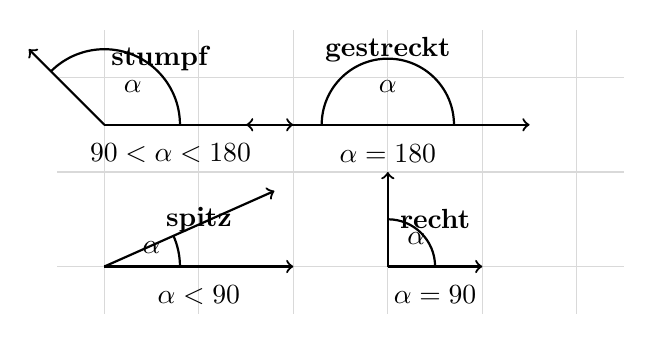
\begin{tikzpicture}[scale=1.2]
  % Koordinatenkreuz
  \draw[thin, gray!30] (-0.5,-0.5) grid (5.5,2.5);
  
  % Winkelarten-Übersicht
  \begin{scope}[shift={(0,0)}]
    \draw[->,thick] (0,0) -- (2,0);
    \draw[->,thick] (0,0) -- (1.8,0.8);
    \draw[thick] (0.8,0) arc (0:24:0.8);
    \node at (0.5,0.2) {$\alpha$};
    \node at (1,0.5) {\textbf{spitz}};
    \node at (1,-0.3) {$\alpha < 90°$};
  \end{scope}
  
  \begin{scope}[shift={(3,0)}]
    \draw[->,thick] (0,0) -- (1,0);
    \draw[->,thick] (0,0) -- (0,1);
    \draw[thick] (0.5,0) arc (0:90:0.5);
    \node at (0.3,0.3) {$\alpha$};
    \node at (0.5,0.5) {\textbf{recht}};
    \node at (0.5,-0.3) {$\alpha = 90°$};
  \end{scope}

  \begin{scope}[shift={(0,1.5)}]
    \draw[->,thick] (0,0) -- (2,0);
    \draw[->,thick] (0,0) -- (-0.8,0.8);
    \draw[thick] (0.8,0) arc (0:135:0.8);
    \node at (0.3,0.4) {$\alpha$};
    \node at (0.6,0.7) {\textbf{stumpf}};
    \node at (0.7,-0.3) {$90° < \alpha < 180°$};
  \end{scope}

  \begin{scope}[shift={(3,1.5)}]
    \draw[->,thick] (0,0) -- (1.5,0);
    \draw[->,thick] (0,0) -- (-1.5,0);
    \draw[thick] (0.7,0) arc (0:180:0.7);
    \node at (0,0.4) {$\alpha$};
    \node at (0,0.8) {\textbf{gestreckt}};
    \node at (0,-0.3) {$\alpha = 180°$};
  \end{scope}
\end{tikzpicture}
\end{center}

\begin{multicols}{2}
\textbf{Winkelarten nach Größe:}
\begin{itemize}
    \item \textbf{Spitzer Winkel:} $0° < \alpha < 90°$
    \item \textbf{Rechter Winkel:} $\alpha = 90°$
    \item \textbf{Stumpfer Winkel:} $90° < \alpha < 180°$
    \item \textbf{Gestreckter Winkel:} $\alpha = 180°$
    \item \textbf{Überstumpfer Winkel:} $180° < \alpha < 360°$
    \item \textbf{Vollständiger Winkel:} $\alpha = 360°$
\end{itemize}

\textbf{Winkelbeziehungen:}
\begin{itemize}
    \item \textbf{Nebenwinkel:} ergänzen sich zu $180°$
    \item \textbf{Scheitelwinkel:} gegenüberliegende Winkel sind gleich groß
    \item \textbf{Komplementärwinkel:} ergänzen sich zu $90°$
    \item \textbf{Supplementärwinkel:} ergänzen sich zu $180°$
\end{itemize}
\end{multicols}

\subsection*{2. Bestimmen von Winkelarten}

\subsubsection*{Aufgabe 2.1: Benenne die Art der folgenden Winkel}

\begin{center}
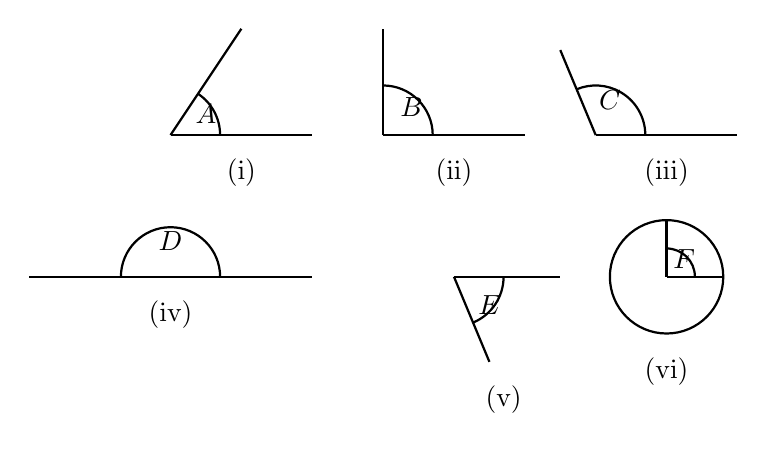
\begin{tikzpicture}[scale=0.9]
    % Winkel A
    \begin{scope}[shift={(0,0)}]
        \draw[thick] (0,0) -- (2,0);
        \draw[thick] (0,0) -- (1,1.5);
        \draw[thick] (0.7,0) arc (0:56:0.7);
        \node at (0.5,0.3) {$A$};
        \node[below] at (1,-0.2) {(i)};
    \end{scope}
    
    % Winkel B
    \begin{scope}[shift={(3,0)}]
        \draw[thick] (0,0) -- (2,0);
        \draw[thick] (0,0) -- (0,1.5);
        \draw[thick] (0.7,0) arc (0:90:0.7);
        \node at (0.4,0.4) {$B$};
        \node[below] at (1,-0.2) {(ii)};
    \end{scope}
    
    % Winkel C
    \begin{scope}[shift={(6,0)}]
        \draw[thick] (0,0) -- (2,0);
        \draw[thick] (0,0) -- (-0.5,1.2);
        \draw[thick] (0.7,0) arc (0:113:0.7);
        \node at (0.2,0.5) {$C$};
        \node[below] at (1,-0.2) {(iii)};
    \end{scope}
    
    % Winkel D
    \begin{scope}[shift={(0,-2)}]
        \draw[thick] (0,0) -- (2,0);
        \draw[thick] (0,0) -- (-2,0);
        \draw[thick] (0.7,0) arc (0:180:0.7);
        \node at (0,0.5) {$D$};
        \node[below] at (0,-0.2) {(iv)};
    \end{scope}
    
    % Winkel E
    \begin{scope}[shift={(4,-2)}]
        \draw[thick] (0,0) -- (1.5,0);
        \draw[thick] (0,0) -- (0.5,-1.2);
        \draw[thick] (0.7,0) arc (0:-67:0.7);
        \node at (0.5,-0.4) {$E$};
        \node[below] at (0.7,-1.4) {(v)};
    \end{scope}
    
    % Winkel F
    \begin{scope}[shift={(7,-2)}]
        \draw[thick] (0,0) circle (0.8);
        \draw[thick] (0,0) -- (0.8,0);
        \draw[thick] (0,0) -- (0,0.8);
        \draw[thick] (0.4,0) arc (0:90:0.4);
        \node at (0.25,0.25) {$F$};
        \node[below] at (0,-1) {(vi)};
    \end{scope}
\end{tikzpicture}
\end{center}

\subsubsection*{Aufgabe 2.2: Markiere alle stumpfen Winkel in der Figur}

\begin{center}
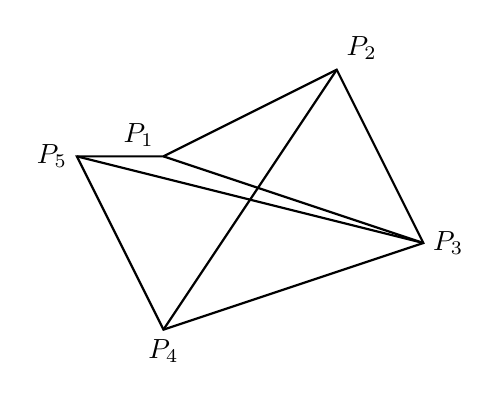
\begin{tikzpicture}[scale=1.1]
    % Stern-ähnliche Figur
    \coordinate (A) at (0,0);
    \coordinate (B) at (2,1);
    \coordinate (C) at (3,-1);
    \coordinate (D) at (0,-2);
    \coordinate (E) at (-1,0);
    
    \draw[thick] (A) -- (B) -- (C) -- (D) -- (E) -- cycle;
    \draw[thick] (A) -- (C);
    \draw[thick] (B) -- (D);
    \draw[thick] (C) -- (E);
    
    % Beschrifte einige Ecken
    \node[above left] at (A) {$P_1$};
    \node[above right] at (B) {$P_2$};
    \node[right] at (C) {$P_3$};
    \node[below] at (D) {$P_4$};
    \node[left] at (E) {$P_5$};
\end{tikzpicture}
\end{center}

\subsection*{3. Winkelbeziehungen an geschnittenen Geraden}

\subsubsection*{Aufgabe 3.1: Benenne die Winkelbeziehungen}

\begin{center}
\begin{tikzpicture}[scale=1.2]
    % Parallele Geraden mit Transversale
    \draw[thick] (-1.5,0) -- (4.5,0) node[right] {$g_1$};
    \draw[thick] (-1.5,2) -- (4.5,2) node[right] {$g_2$};
    \draw[thick] (0,-0.5) -- (3,3) node[above] {$t$};
    
    % Schnittpunkte
    \coordinate (P1) at (1,0);
    \coordinate (P2) at (2,2);
    
    % Winkel markieren
    \draw[thick] ($(P1)+(0.6,0)$) arc (0:56:0.6) node[midway, right] {$\alpha$};
    \draw[thick] ($(P1)+(0.5,0)$) arc (180:124:0.5) node[midway, left] {$\beta$};
    \draw[thick] ($(P2)+(0,0.5)$) arc (270:304:0.5) node[midway, below left] {$\gamma$};
    \draw[thick] ($(P2)+(0,0.5)$) arc (90:124:0.5) node[midway, above left] {$\delta$};
    
    % Punkte markieren
    \fill (P1) circle (2pt) node[below] {$P_1$};
    \fill (P2) circle (2pt) node[above] {$P_2$};
\end{tikzpicture}
\end{center}

\subsubsection*{Aufgabe 3.2: Berechne die fehlenden Winkel}

\begin{center}
\begin{tikzpicture}[scale=1.1]
    % Kreuzende Geraden
    \draw[thick] (-1.5,-1.5) -- (3,3) node[right] {$g$};
    \draw[thick] (-1.5,2) -- (3,-2.5) node[right] {$h$};
    
    % Schnittpunkt
    \coordinate (S) at (0.75,0.75);
    \fill (S) circle (2pt) node[above right] {$S$};
    
    % Winkel markieren
    \draw[thick] ($(S)+(0.6,0)$) arc (0:125:0.6);
    \node at (0.3,0.3) {$130°$};
    
    \draw[thick] ($(S)+(0,0.6)$) arc (90:235:0.6);
    \node at (-0.2,0.3) {$\alpha$};
    
    \draw[thick] ($(S)+(0,-0.6)$) arc (-90:35:0.6);
    \node at (0.3,-0.2) {$\beta$};
\end{tikzpicture}
\end{center}

\subsubsection*{Aufgabe 3.3: Bestimme alle Winkel in der Figur}
Gegeben ist der Winkel $\alpha = 35°$.

\begin{center}
\begin{tikzpicture}[scale=1.2]
    % Parallel- und Transversallinien
    \draw[thick] (-1,0) -- (4,0) node[right] {$g_1$};
    \draw[thick] (-1,2) -- (4,2) node[right] {$g_2$};
    \draw[thick] (0,-0.5) -- (2,3) node[above] {$t_1$};
    \draw[thick] (3,-0.5) -- (1,3) node[above] {$t_2$};
    
    % Schnittpunkte
    \coordinate (P1) at (0.67,0);
    \coordinate (P2) at (1.33,2);
    \coordinate (P3) at (2.33,0);
    \coordinate (P4) at (1.67,2);
    
    % Winkel markieren
    \draw[thick] ($(P1)+(0.5,0)$) arc (0:75:0.5);
    \node at (0.83,0.25) {$\alpha$};
    
    % Punkte markieren
    \fill (P1) circle (1.5pt) node[below] {$A$};
    \fill (P2) circle (1.5pt) node[above] {$B$};
    \fill (P3) circle (1.5pt) node[below] {$C$};
    \fill (P4) circle (1.5pt) node[above] {$D$};
\end{tikzpicture}
\end{center}

\subsection*{4. Winkel in geometrischen Figuren}

\subsubsection*{Aufgabe 4.1: Berechne die Innenwinkel der Dreiecke}
Bestimme alle Innenwinkel in diesen Dreiecken:

\begin{center}
\begin{tikzpicture}[scale=0.9]
    % Dreieck 1
    \begin{scope}[shift={(-3,0)}]
        \coordinate (A) at (0,0);
        \coordinate (B) at (3,0);
        \coordinate (C) at (1.5,2.5);
        \draw[thick] (A) -- (B) -- (C) -- cycle;
        
        % Winkel markieren
        \draw[thick] ($(A)+(0.6,0)$) arc (0:40:0.6);
        \node at (0.5,0.2) {$30°$};
        \draw[thick] ($(B)+(-0.6,0)$) arc (180:150:0.6);
        \node at (2.5,0.2) {$40°$};
        
        \node[below] at (1.5,-0.5) {Dreieck 1};
    \end{scope}

    % Dreieck 2
    \begin{scope}[shift={(3,0)}]
        \coordinate (A) at (0,0);
        \coordinate (B) at (3,0);
        \coordinate (C) at (3,2);
        \draw[thick] (A) -- (B) -- (C) -- cycle;
        
        % Winkel markieren
        \draw[thick] ($(B)+(0,0.6)$) arc (90:180:0.6);
        \node at (2.7,0.3) {$90°$};
        \draw[thick] ($(A)+(0.6,0)$) arc (0:34:0.6);
        \node at (0.5,0.2) {$\alpha$};
        
        \node[below] at (1.5,-0.5) {Dreieck 2};
    \end{scope}
\end{tikzpicture}
\end{center}

\subsubsection*{Aufgabe 4.2: Winkel im Viereck}
Bestimme alle Innenwinkel im Viereck:

\begin{center}
\begin{tikzpicture}[scale=1]
    \coordinate (A) at (0,0);
    \coordinate (B) at (4,0);
    \coordinate (C) at (3,2);
    \coordinate (D) at (1,3);
    
    \draw[thick] (A) -- (B) -- (C) -- (D) -- cycle;
    
    % Winkel markieren
    \draw[thick] ($(A)+(0.7,0)$) arc (0:37:0.7);
    \node at (0.5,0.2) {$\alpha$};
    \draw[thick] ($(B)+(-0.7,0)$) arc (180:210:0.7);
    \node at (3.5,0.2) {$135°$};
    \draw[thick] ($(C)+(-0.4,-0.6)$) arc (-125:-220:0.7);
    \node at (2.7,1.7) {$110°$};
\end{tikzpicture}
\end{center}

\subsection*{5. Anwendungsaufgaben}

\subsubsection*{Aufgabe 5.1: Uhrzeigerwinkel}
Der Stundenzeiger und der Minutenzeiger einer Uhr bilden einen Winkel miteinander. Wie groß ist dieser Winkel zu den angegebenen Uhrzeiten?

\begin{center}
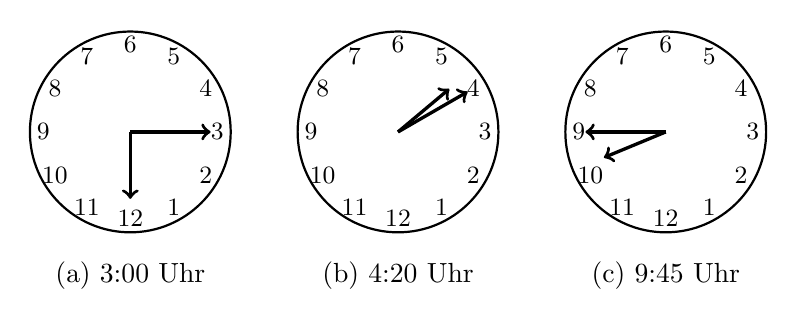
\begin{tikzpicture}[scale=0.85]
    % Uhr 1: 3 Uhr
    \begin{scope}[shift={(-3,0)}]
        \draw[thick] (0,0) circle (1.5);
        \foreach \i in {1,...,12} {
            \node[font=\small] at ({1.3*cos(30*\i-90)}, {1.3*sin(30*\i-90)}) {\i};
        }
        \draw[very thick, ->] (0,0) -- ({1.0*cos(0*30-90)}, {1.0*sin(0*30-90)});
        \draw[very thick, ->] (0,0) -- ({1.2*cos(3*30-90)}, {1.2*sin(3*30-90)});
        \node[below] at (0,-1.8) {(a) 3:00 Uhr};
    \end{scope}

    % Uhr 2: 4:20
    \begin{scope}[shift={(1,0)}]
        \draw[thick] (0,0) circle (1.5);
        \foreach \i in {1,...,12} {
            \node[font=\small] at ({1.3*cos(30*\i-90)}, {1.3*sin(30*\i-90)}) {\i};
        }
        \draw[very thick, ->] (0,0) -- ({1.0*cos(4*30-90+20*0.5)}, {1.0*sin(4*30-90+20*0.5)});
        \draw[very thick, ->] (0,0) -- ({1.2*cos(4*30-90)}, {1.2*sin(4*30-90)});
        \node[below] at (0,-1.8) {(b) 4:20 Uhr};
    \end{scope}
    
    % Uhr 3: 9:45
    \begin{scope}[shift={(5,0)}]
        \draw[thick] (0,0) circle (1.5);
        \foreach \i in {1,...,12} {
            \node[font=\small] at ({1.3*cos(30*\i-90)}, {1.3*sin(30*\i-90)}) {\i};
        }
        \draw[very thick, ->] (0,0) -- ({1.0*cos(9*30-90+45*0.5)}, {1.0*sin(9*30-90+45*0.5)});
        \draw[very thick, ->] (0,0) -- ({1.2*cos(9*30-90)}, {1.2*sin(9*30-90)});
        \node[below] at (0,-1.8) {(c) 9:45 Uhr};
    \end{scope}
\end{tikzpicture}
\end{center}

\subsubsection*{Aufgabe 5.2: Winkel in Alltagssituationen}

\begin{center}
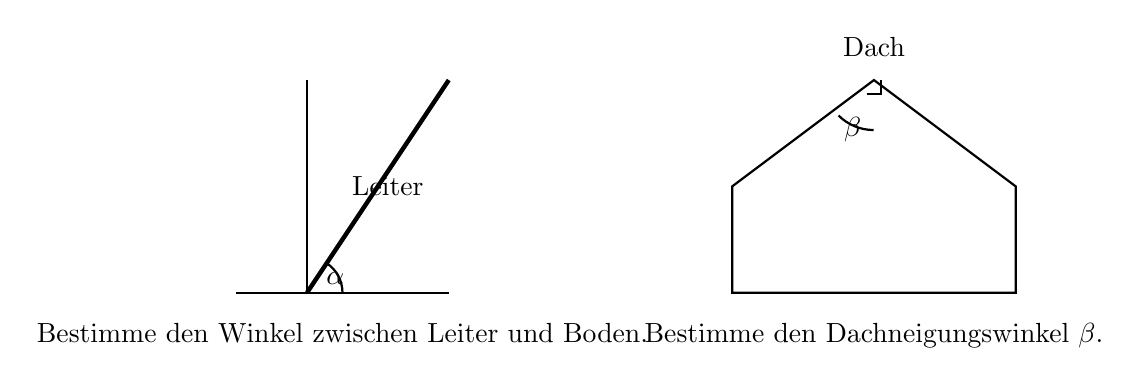
\begin{tikzpicture}[scale=0.9]
    % Leiter an Wand
    \begin{scope}[shift={(-3,0)}]
        % Boden und Wand
        \draw[thick] (-1,0) -- (2,0);
        \draw[thick] (0,0) -- (0,3);
        
        % Leiter
        \draw[ultra thick] (0,0) -- (2,3);
        
        % Winkel markieren
        \draw[thick] (0.5,0) arc (0:56:0.5);
        \node at (0.4,0.2) {$\alpha$};
        
        % Beschriftung
        \node[right] at (0.5,1.5) {Leiter};
        \node[below] at (0.5,-0.3) {Bestimme den Winkel zwischen Leiter und Boden.};
    \end{scope}

    % Dach
    \begin{scope}[shift={(3,0)}]
        % Haus
        \draw[thick] (0,0) -- (0,1.5) -- (2,3) -- (4,1.5) -- (4,0) -- cycle;
        
        % Winkel markieren
        \draw[thick] (1.9,2.8) -- (2.1,2.8) -- (2.1,3);
        \draw[thick] (1.5,2.5) arc (225:270:0.7);
        \node at (1.7,2.3) {$\beta$};
        
        % Beschriftung
        \node[above] at (2,3.2) {Dach};
        \node[below] at (2,-0.3) {Bestimme den Dachneigungswinkel $\beta$.};
    \end{scope}
\end{tikzpicture}
\end{center}

\subsection*{6. Kreatives Anwendungsprojekt}

\subsubsection*{Aufgabe 6.1: Winkelarten in der Kunst}

Untersuche das folgende Kunstwerk und bestimme:
\begin{itemize}
    \item Alle rechten Winkel (markiere in blau)
    \item Alle stumpfen Winkel (markiere in rot)
    \item Alle spitzen Winkel (markiere in grün)
\end{itemize}

\begin{center}
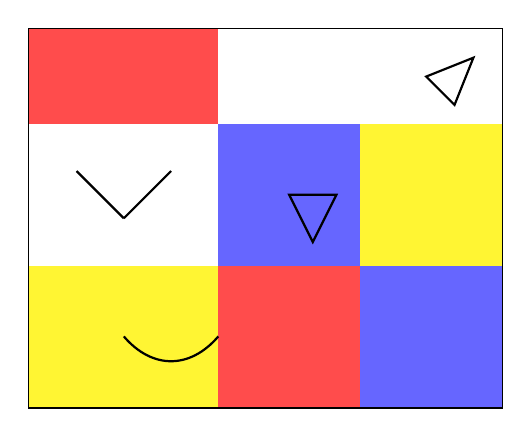
\begin{tikzpicture}[scale=1.2]
    % Mondrian-inspiriertes Kunstwerk
    \draw[very thick] (0,0) rectangle (5,4);
    \draw[very thick] (0,1.5) -- (5,1.5);
    \draw[very thick] (0,3) -- (5,3);
    \draw[very thick] (2,0) -- (2,4);
    \draw[very thick] (3.5,0) -- (3.5,4);
    
    % Farbige Flächen (Mondrian-Stil)
    \fill[yellow!80] (0,0) rectangle (2,1.5);
    \fill[red!70] (2,0) rectangle (3.5,1.5);
    \fill[blue!60] (3.5,0) rectangle (5,1.5);
    \fill[white] (0,1.5) rectangle (2,3);
    \fill[blue!60] (2,1.5) rectangle (3.5,3);
    \fill[yellow!80] (3.5,1.5) rectangle (5,3);
    \fill[red!70] (0,3) rectangle (2,4);
    \fill[white] (2,3) rectangle (3.5,4);
    \fill[white] (3.5,3) rectangle (5,4);
    
    % Externe Elemente für die Übung
    \draw[thick] (1,2) -- (1.5,2.5);
    \draw[thick] (1,2) -- (0.5,2.5);
    
    \draw[thick] (4.2,3.5) -- (4.7,3.7) -- (4.5,3.2) -- cycle;
    
    \draw[thick] (2.75,2.25) -- (3.25,2.25) -- (3,1.75) -- cycle;
    
    \draw[thick] (1,0.75) .. controls (1.3,0.4) and (1.7,0.4) .. (2,0.75);
\end{tikzpicture}
\end{center}

\subsection*{7. Lösungen zu ausgewählten Aufgaben}

\begin{multicols}{2}
\subsubsection*{Lösung zu 2.1:}
(i) Spitzer Winkel\\
(ii) Rechter Winkel\\
(iii) Stumpfer Winkel\\
(iv) Gestreckter Winkel\\
(v) Spitzer Winkel (negative Zählung)\\
(vi) Rechter Winkel

\columnbreak

\subsubsection*{Lösung zu 3.2:}
Wenn ein Winkel $130°$ beträgt, dann sind die anderen beiden Winkel:\\
$\alpha = 180° - 130° = 50°$\\
$\beta = 180° - 130° = 50°$\\
(Scheitelwinkel sind gleich)
\end{multicols}

\begin{multicols}{2}
\subsubsection*{Lösung zu 4.1:}
Dreieck 1: $30° + 40° + \gamma = 180°$\\
Also: $\gamma = 180° - 30° - 40° = 110°$

\columnbreak

\subsubsection*{Lösung zu 5.1:}
(a) 3:00 Uhr: $90°$\\
(b) 4:20 Uhr: $130°$\\
(c) 9:45 Uhr: $7,5°$
\end{multicols}

\subsubsection*{Hinweis zur Aufgabe 5.1:}
Der Winkel zwischen Stunden- und Minutenzeiger lässt sich berechnen mit:
$$ \text{Winkel} = \left| 30 \cdot \text{Stunden} - 6 \cdot \text{Minuten} + 0,5 \cdot \text{Minuten} \right| $$